\documentclass[11pt,a4paper]{article}

% ---------------------------------------------------------------
% Packages (house style: Nat Comms draft)
% ---------------------------------------------------------------
\usepackage[utf8]{inputenc}
\usepackage[T1]{fontenc}
\usepackage{mathptmx}
\usepackage{geometry}
\geometry{a4paper, top=30mm, bottom=30mm, left=30mm, right=30mm}
\usepackage{amsmath,amssymb}
\usepackage{graphicx}
\usepackage{booktabs}
\usepackage{array}
\usepackage{caption}
\usepackage{float}
\usepackage{microtype}
\usepackage[numbers,super,sort&compress]{natbib}
\usepackage[colorlinks=true,linkcolor=blue,citecolor=blue,urlcolor=blue]{hyperref}
\usepackage{setspace}
\usepackage{titlesec}
\usepackage{parskip}

\onehalfspacing
\titleformat{\section}{\large\bfseries}{}{0em}{}
\titleformat{\subsection}{\normalsize\bfseries}{}{0em}{}
\titleformat{\subsubsection}{\normalsize\itshape}{}{0em}{}
\graphicspath{{../results/bell_qnn/}}

% Every number below that comes from a sweep is generated from results/bell_qnn/*.json by fill_macros.py
% generated by fill_macros.py -- do not edit
\newcommand{\MultTwo}{$2.6$}  % sd 0.47, n=10
\newcommand{\MultThree}{$4.8$}  % sd 1.09, n=10
\newcommand{\MultFour}{$7.8$}  % sd 1.57, n=10
\newcommand{\MultFive}{$16.6$}  % sd 2.96, n=10
\newcommand{\MultSix}{$32$}  % sd 4.48, n=10
\newcommand{\MultSeven}{$76$}  % sd 7.89, n=10
\newcommand{\MultEight}{$191$}  % sd 28.09, n=10
\newcommand{\GlobTwo}{$2.0$}  % sd 0.25, n=10
\newcommand{\BoundTwo}{$12.2$}
\newcommand{\BoundInfTwo}{$12.2$}
\newcommand{\ExactTwo}{$3.2$}
\newcommand{\ExactInfTwo}{$3.1$}
\newcommand{\GlobThree}{$2.7$}  % sd 0.29, n=10
\newcommand{\BoundThree}{$20$}
\newcommand{\BoundInfThree}{$19.8$}
\newcommand{\ExactThree}{$4.9$}
\newcommand{\ExactInfThree}{$4.5$}
\newcommand{\GlobFour}{$3.8$}  % sd 0.42, n=10
\newcommand{\BoundFour}{$46$}
\newcommand{\BoundInfFour}{$45$}
\newcommand{\ExactFour}{$10.1$}
\newcommand{\ExactInfFour}{$8.7$}
\newcommand{\GlobFive}{$4.9$}  % sd 0.65, n=10
\newcommand{\BoundFive}{$82$}
\newcommand{\BoundInfFive}{$78$}
\newcommand{\ExactFive}{$16.3$}
\newcommand{\ExactInfFive}{$10.8$}
\newcommand{\GlobSix}{$7.0$}  % sd 0.60, n=10
\newcommand{\BoundSix}{$184$}
\newcommand{\BoundInfSix}{$170$}
\newcommand{\ExactSix}{$37$}
\newcommand{\ExactInfSix}{$18.5$}
\newcommand{\GlobSeven}{$10.6$}  % sd 1.48, n=10
\newcommand{\BoundSeven}{$365$}
\newcommand{\BoundInfSeven}{$311$}
\newcommand{\ExactSeven}{$81$}
\newcommand{\ExactInfSeven}{$24$}
\newcommand{\GlobEight}{$19.3$}  % sd 1.49, n=10
\newcommand{\BoundEight}{$895$}
\newcommand{\BoundInfEight}{$704$}
\newcommand{\ExactEight}{$213$}
\newcommand{\ExactInfEight}{$42$}
\newcommand{\PanelBsentence}{Over the measured range the single-copy RMSE falls as $C^{-0.60}$ between $C=100$ and $800$ and as $C^{-0.65}$ from $C=1600$ until it reaches the coherent reader, faster than $C^{-1/2}$, because clipping to the physical range removes a share of the error that shrinks as estimates move back inside it; the coherent reader follows $C^{-0.52}$ throughout.}
\newcommand{\CampaignRows}{%
0 & 0.0510 & 0.1946 & 0.3861 & $-0.1437$ \\
1 & 0.0501 & 0.2011 & 0.3365 & $-0.1509$ \\
7 & 0.0521 & 0.1931 & 0.3546 & $-0.1411$ \\
42 & 0.0505 & 0.1942 & 0.3127 & $-0.1437$ \\
123 & 0.0530 & 0.1924 & 0.3439 & $-0.1394$ \\
456 & 0.0526 & 0.1966 & 0.3621 & $-0.1440$ \\
789 & 0.0491 & 0.2007 & 0.3208 & $-0.1516$ \\
1234 & 0.0498 & 0.1797 & 0.3198 & $-0.1299$ \\
2024 & 0.0509 & 0.1943 & 0.3249 & $-0.1434$ \\
3407 & 0.0518 & 0.1907 & 0.3339 & $-0.1389$ \\}
\newcommand{\EmulatedBlock}{%
\begin{table}[H]\centering\small
\caption{Transpiled emulation on the IBM Heron r2 model \texttt{FakeFez}, $C=400$ copies per state, $n=2|A|$; RMSE of $\mathrm{tr}(\rho_A^2)$, mean (s.d.) over official seeds. 2q gates: mean two-qubit gate count after transpilation (Bell / one single-copy circuit). Wins: seeds in which the self-calibrated Bell reader beats the single-copy reader.}
\label{tab:emu}
\begin{tabular}{rlrrrrrr}
\toprule
$|A|$ & Noise & Seeds & Bell raw & Bell calibrated & Single-copy & 2q gates & Wins \\
\midrule
2 & FakeFez noise & 10 & 0.077 (0.006) & 0.060 (0.007) & 0.089 (0.006) & 41 / 12 & 10/10 \\
2 & ideal & 10 & 0.049 (0.005) & 0.049 (0.005) & 0.077 (0.007) & 41 / 12 & 10/10 \\
3 & FakeFez noise & 10 & 0.108 (0.007) & 0.077 (0.006) & 0.138 (0.013) & 69 / 19 & 10/10 \\
\bottomrule
\end{tabular}
\end{table}

At $|A|=2$ the self-calibrated coherent reader reaches an RMSE of $0.060$ against $0.089$ for the single-copy reader (factor $1.5$, lower in 10 of 10 seeds, exact Wilcoxon $p=0.00098$); uncorrected it reaches $0.077$, and the calibration constant is $\lambda=0.949$ per qubit. At $|A|=3$ the self-calibrated coherent reader reaches an RMSE of $0.077$ against $0.138$ for the single-copy reader (factor $1.8$, lower in 10 of 10 seeds, exact Wilcoxon $p=0.00098$); uncorrected it reaches $0.108$, and the calibration constant is $\lambda=0.945$ per qubit. The Bell circuit is several times deeper in two-qubit gates than a single-copy circuit, because it prepares two copies and routes the pairwise CNOTs on heavy-hex; its estimate nevertheless stays ahead in every seed once the shared contraction is calibrated out.}
\newcommand{\EmulatedAbstract}{survives transpilation and calibrated noise on an emulated IBM Heron device (RMSE $0.077$ against $0.138$ at $|A|=3$, 10 of 10 seeds).}


\begin{document}

\begin{center}
{\Large\bfseries How many copies is coherence worth?\\[0.3em]
Exact exchange rates between two-copy and single-copy\\
readout of quantum data}

\vspace{1.2em}

% TODO(authors): fill in the author list and affiliations before circulation.
[Author list to be completed]

\end{center}

\vspace{0.5em}

% ---------------------------------------------------------------
\noindent\textbf{Abstract.}\quad
Coherent access to two copies of a quantum state estimates nonlinear properties with far fewer
measurements than single-copy readout, but how many fewer \emph{state preparations} it saves is
usually stated asymptotically or as an upper bound, not at the budget of an experiment. We measure and predict this exchange rate for the purity
$\mathrm{tr}(\rho_A^2)$ of a subsystem, the building block of R\'enyi entropies and of
concentratable entanglement. At $C=400$ copies per state and $|A|=4$, two-copy Bell sampling
reaches an RMSE of $0.051$ against $0.194$ for the strongest local single-copy reader, in all ten
pre-registered seeds (exact Wilcoxon $p=9.8\times10^{-4}$, Holm-adjusted $0.002$). To match the
coherent reader, local randomized measurements need \MultFour\ times more copies at $|A|=4$ and
\MultEight\ at $|A|=8$; global random measurements, which scale better with the dimension,
still need \GlobEight. Evaluating the known U-statistic variance
decomposition exactly, instead of bounding it, predicts these rates without fitted parameters and
shows that the published bound overstates them four- to fivefold at our budget and up to
seventeenfold asymptotically (\BoundInfEight\ against \ExactInfEight\ at $|A|=8$). The rate depends on the budget: it is largest where experiments
operate and grows as $\approx2.7^{|A|}/\sqrt{C}$ there. The advantage persists when the label must
be learned (circuit depth, von Neumann entropy), on the NTangled dataset, under exact depolarising
and readout noise, where both readers share the bias but only the coherent one calibrates itself for
free, and on an emulated IBM Heron device with calibrated noise.

\vspace{0.4em}
\noindent\textbf{Keywords:} quantum data, randomized measurements, classical shadows, Bell sampling,
sample complexity, purity, entanglement.

\hrule
\vspace{0.6em}

% ---------------------------------------------------------------
\section{Introduction}

Machine learning on quantum data has a currency problem. Two readers of a quantum state can be
compared at equal shots, equal parameters or equal circuit depth, and the choice decides the
outcome. Separations that survive scrutiny are stated in \emph{copies}, the number of times the
unknown state is prepared, because that is what a single-copy device and a coherent multi-copy
device both consume \citep{huang2021advantage,isogai2026pac}. Classical shadows predict many
properties from few single-copy measurements \citep{huang2020predicting}, classical learners on
shadows are provably efficient for broad classes of many-body problems \citep{huang2021provably},
and quantum convolutional networks on standard phase datasets are effectively simulable from Pauli
shadows \citep{bermejo2024qcnn}. A single-copy baseline is therefore not optional.

Nonlinear functionals are where the currency bites. Randomized measurements estimate R\'enyi-2
entropies from correlations between single-copy outcomes
\citep{brydges2019probing,elben2019statistical,elben2022toolbox}; the variance of the resulting
U-statistic splits into a term linear and a term quadratic in the snapshots, with published upper
bounds exponential in the subsystem size \citep{elben2020mixed}. The optimal single-copy sample
complexity of purity estimation scales as $\sqrt d$ \citep{gong2024purity,liu2026moments}, whereas
the swap observable measured transversally on two copies estimates it at a cost independent of the
dimension (Methods). One extra replica gives exponential savings for nonlinear properties
\citep{ye2025replica}, an infinite hierarchy of multi-copy tasks exists \citep{noeller2025hierarchy},
conjugate states and minimal quantum memory recover part of the gain \citep{king2024conjugate}, and
purification with constant ancillas gives exponential separations \citep{liu2024purification}. In
the other direction, quantum PAC learning gains require inverse access to the preparation
\citep{isogai2026pac} and bound entanglement does not suffice for an exponential learning advantage
\citep{kang2026bound}. Experiments have demonstrated multi-copy neural networks on two qubits
\citep{tulewicz2024multicopy} and entanglement-enhanced learning on up to sixteen qubits
\citep{seif2024entanglement}; two-copy shadow tomography has been evaluated for estimation rather
than learning \citep{tran2025two}, and learning with optimal similarity measurements
\citep{li2026similarity} and phase classification from partial tomography \citep{tanji2025phase}
have been proposed.

These results are asymptotic statements, upper bounds, or comparisons at unequal budgets. A
practitioner who must decide whether to spend a qubit register on a second copy needs a number: at
the budget available, for the subsystem of interest, how many single-copy preparations does
coherence replace? We provide that number for local and global single-copy readers, show how to
predict it exactly from the state ensemble, and test whether it survives learning, a published
dataset, noise and compilation to a current device.

\textbf{Contributions.} (i) A pre-registered equal-copy comparison against the strongest
single-copy readers we could build, local and global. (ii) A measured exchange rate for $|A|=2$ to
$8$, together with an exact evaluation of the U-statistic variance for the actual ensemble which
predicts it without fitted parameters, shows that the published bounds overstate it severalfold, and
makes explicit that it depends on the budget. (iii) Evidence that the advantage survives when a
learner must combine features into a label no reader estimates directly, and on NTangled at equal
copies. (iv) An exact noise study and a transpiled, calibrated emulation on an IBM Heron model, with a
copy and circuit budget for a hardware run. (v) An audited protocol whose corrections are reported.

\subsection*{Research questions}
\textbf{RQ1.} At equal copies, how much more accurately does a two-copy reader estimate subsystem
purity than the strongest local single-copy reader?\\
\textbf{RQ2.} How many single-copy preparations does coherence replace, as a function of $|A|$, of
the budget and of the single-copy reader, and can the number be predicted?\\
\textbf{RQ3.} Does the advantage survive when the label must be learned, and on a published
dataset?\\
\textbf{RQ4.} Does it survive realistic noise and compilation to a current device?

% ---------------------------------------------------------------
\section{Results}

\subsection{Readers and budget}

All readers receive the same $C$ copies of each state. The \emph{coherent reader} measures $C/2$
pairs transversally in the Bell basis; the product of swap signs over a window $W$ is a $\pm1$
variable whose mean is $\mathrm{tr}(\rho_W^2)$, and one sample set yields every window purity at
once (Methods). The \emph{local single-copy reader} measures each copy in a random local Pauli
basis and estimates the purity with the unbiased U-statistic over pairs of snapshots
\citep{huang2020predicting,elben2022toolbox}. One shot per basis, clipped to the physical range
$[2^{-|A|},1]$, is its most copy-efficient configuration in our tests (Supplementary
Table~\ref{tab:rivals}); the grouped configuration with ten shots per basis, common on hardware, is
reported alongside. The \emph{global single-copy reader} applies a Haar-random unitary to all of $A$
before each one-shot measurement; it has the better dimension scaling but requires an entangling
circuit across $A$, whereas both the local and the Bell reader use depth-one measurement circuits.
States are brickwork circuits of depth one to four with Haar two-qubit gates on $n=2|A|$ qubits,
and $A$ is the left half.

\subsection{Confirmatory comparison}

Ten seeds fixed in advance, $400$ states each, at $|A|=4$ and $C=400$
(Table~\ref{tab:campaign}). The coherent reader reaches an RMSE of $0.049$--$0.053$; the strongest
local single-copy reader reaches $0.180$--$0.201$. The paired difference is $-0.143$ (s.d.\
$0.006$), negative in all ten seeds; the exact one-sided Wilcoxon test gives $p=9.8\times10^{-4}$,
the smallest value attainable with ten seeds, and Holm correction over the pre-registered two-idea
family gives $0.002$. Against the grouped reader the factor is $6.6$ instead of $3.8$. The
campaign passes in all ten seeds on PennyLane and on Qiskit, whose Bell probabilities agree to
$2.2\times10^{-16}$.

\begin{table}[H]
\centering
\small
\caption{Confirmatory campaign: RMSE of $\mathrm{tr}(\rho_A^2)$ at $C=400$, $|A|=4$, $n=8$,
$400$ states per seed. ``Strongest'' is the minimum over the local single-copy readers (in every
seed, one shot per basis, clipped); ``grouped'' is the pre-registered ten-shot reader.}
\label{tab:campaign}
\begin{tabular}{rrrrr}
\toprule
Seed & Two-copy Bell & Strongest single-copy & Grouped ($S=10$) & Difference \\
\midrule
\CampaignRows
\midrule
Mean & 0.0511 & 0.1937 & 0.3395 & $-0.1426$ \\
\bottomrule
\end{tabular}
\end{table}

\subsection{The exchange rate}

Figure~\ref{fig:scale}a sweeps $|A|=2,\dots,8$ at $C=400$ ($n$ up to $16$, ten seeds). The coherent
reader stays at $0.048$--$0.052$. The local reader degrades from $0.078$ to saturation near the
physical bound and is worse than a constant predictor from $|A|=5$. The global reader degrades more
slowly, from $0.071$ to $0.44$. Converting these errors into copies requires care, because the
single-copy curves are not parallel to the coherent one (panel b): \PanelBsentence\ We therefore
measure the copies each reader needs on a grid of budgets and interpolate (panel c). Matching the
coherent reader at $C=400$ takes the local reader \MultTwo, \MultThree, \MultFour, \MultFive,
\MultSix, \MultSeven\ and \MultEight\ times more copies for $|A|=2,\dots,8$, and the global reader
\GlobTwo, \GlobThree, \GlobFour, \GlobFive, \GlobSix, \GlobSeven\ and \GlobEight\ times more.
Coherence therefore beats every non-adaptive single-copy reader we tested at every size, by a
factor that grows with the subsystem; the global reader's slower growth is consistent with the
$\sqrt d$ scaling of optimal single-copy purity estimation \citep{gong2024purity,liu2026moments}.

\begin{figure}[H]
\centering
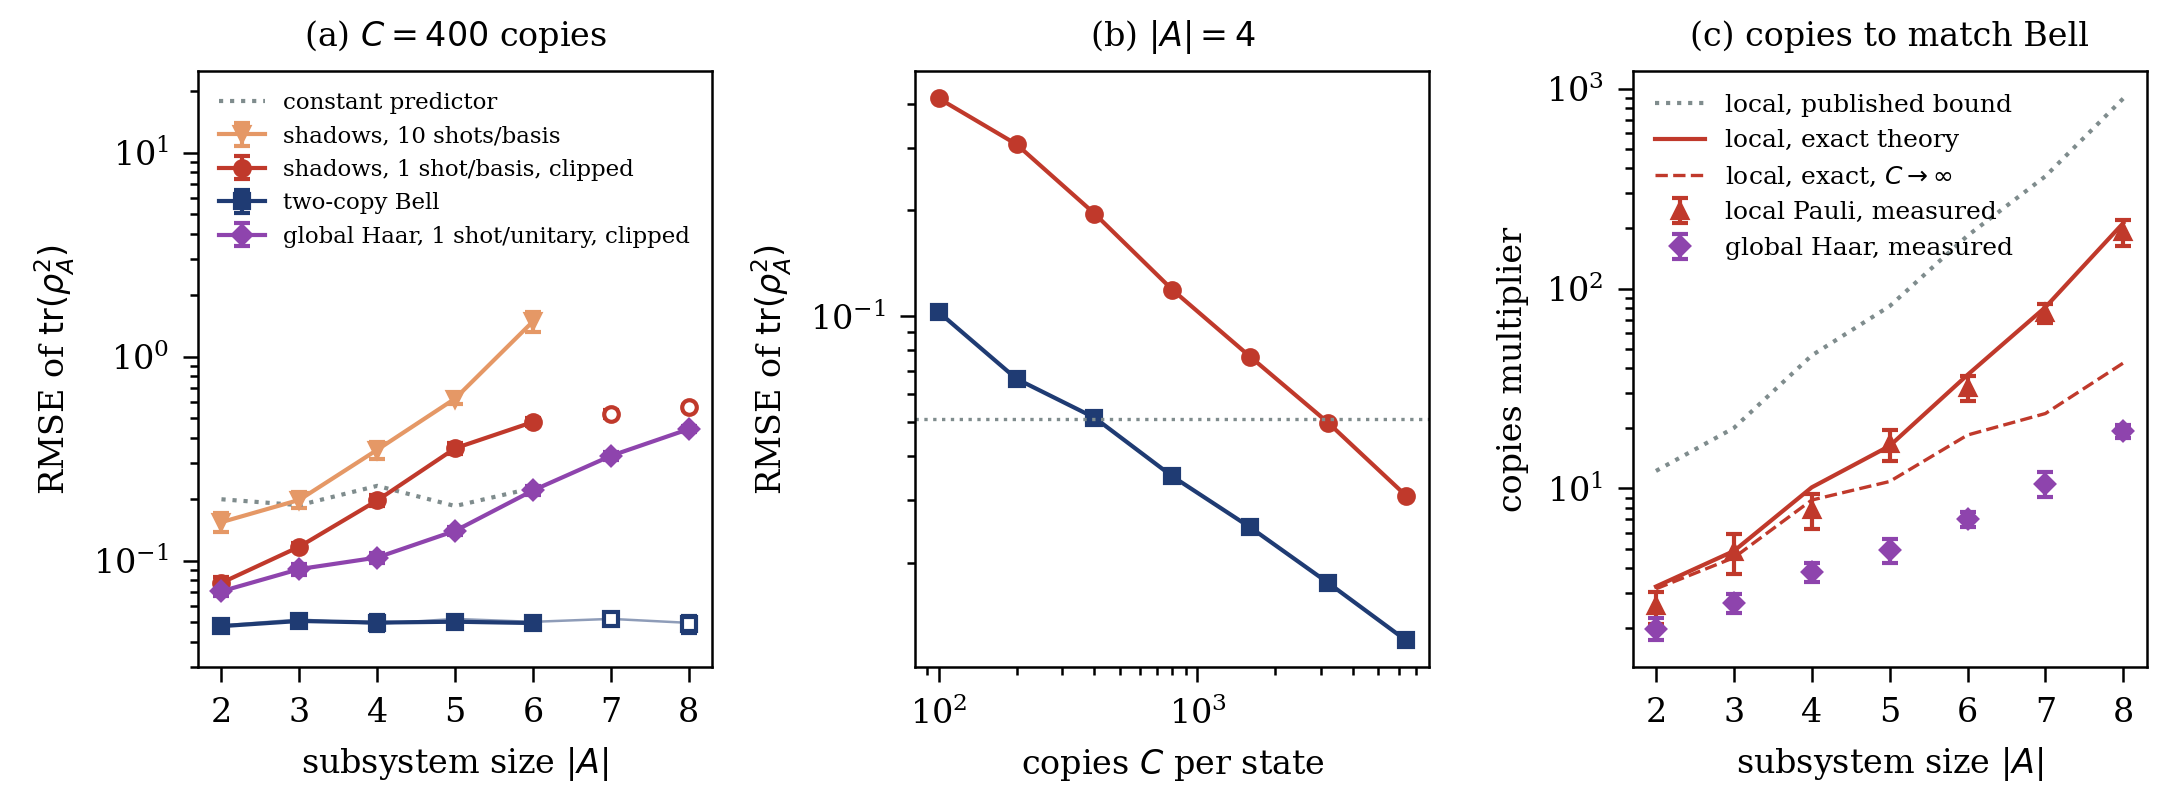
\includegraphics[width=\textwidth]{fig1_scale.png}
\caption{The exchange rate. (a) RMSE of $\mathrm{tr}(\rho_A^2)$ against subsystem size at $C=400$;
mean and s.d.\ over ten seeds; open markers at $|A|=7,8$ come from the copies sweep on the same
states; thin line: closed-form coherent prediction; dotted: constant predictor. (b) RMSE against
copies at $|A|=4$; the dotted line marks the coherent reader at $C=400$. (c) Copies a single-copy
reader needs to reach the coherent reader's RMSE at $C=400$: measured on a grid of budgets and
interpolated (markers; mean and s.d.\ over ten seeds), exact theory for the local reader at $C=400$
(solid) and $C\to\infty$ (dashed), Eq.~\eqref{eq:rate}, and the rate implied by the published variance
bound \citep{elben2020mixed} (dotted).}
\label{fig:scale}
\end{figure}

\textbf{Exact prediction.} The coherent estimator is the mean of $C/2$ independent signs, so
$\mathrm{Var}_{\mathrm B}=2(1-p^2)/C$ with $p=\mathrm{tr}(\rho_A^2)$, independent of $|A|$. The local
estimator is a second-order U-statistic over $M$ snapshots with kernel
$h(x,y)=\mathrm{tr}(\hat\sigma_x\hat\sigma_y)$, and its variance has the standard decomposition
\citep{elben2020mixed}
\begin{equation}
\mathrm{Var}_{\mathrm S}(M)=\frac{4(M-2)}{M(M-1)}\,\zeta_1+\frac{2}{M(M-1)}\,\zeta_2,\qquad
\zeta_1=\mathrm{Var}_x\,\mathrm{tr}(\hat\sigma_x\rho_A),\quad \zeta_2=\mathrm{Var}_{x,y}\,h(x,y).
\label{eq:var}
\end{equation}
Ref.~\citenum{elben2020mixed} bounds the two terms by $\zeta_1\le2^{|A|}p$ and
$\zeta_2\le2\cdot8^{|A|}$. We instead evaluate them exactly for every state, as contractions of the
$6^{|A|}$ table of snapshot probabilities (Methods). Equating dataset-averaged variances gives the
exchange rate $m=M/C$,
\begin{equation}
m\;\simeq\;\begin{cases}
\sqrt{\overline{\zeta_2}\,/\,\big(\overline{1-p^2}\;C\big)} & M\ll M^\ast=\zeta_2/2\zeta_1,\\[0.3em]
2\,\overline{\zeta_1}\,/\,\overline{1-p^2} & M\gg M^\ast,
\end{cases}
\label{eq:rate}
\end{equation}
solved exactly by root finding in practice. Without fitted parameters, the predicted RMSE at
$C=400$ matches the simulated one within $4\%$ for both readers at every $|A|=2,\dots,6$, and the
predicted rates (\ExactTwo, \ExactThree, \ExactFour, \ExactFive, \ExactSix, \ExactSeven,
\ExactEight) agree with the measured ones within $30\%$, lying above them in six of seven sizes
because clipping only helps the measured reader.

Two consequences follow. First, the published bound is loose for this ensemble: it implies
\BoundFour\ instead of \ExactFour\ at $|A|=4$ and \BoundEight\ instead of \ExactEight\ at $|A|=8$, and
\BoundInfEight\ instead of \ExactInfEight\ asymptotically. Over our states $\zeta_2$ grows by $7.2$
per qubit, close to the second moment of the single-qubit kernel, which equals $7$ for a maximally
mixed qubit, against $8$ in the bound; $\zeta_1$ grows by only $1.4$--$1.8$, against $2$. Second,
the rate depends on the budget. The crossover $M^\ast$ rises from $35$ snapshots at $|A|=2$ to
$3.4\times10^{5}$ at $|A|=8$, so beyond $|A|\approx4$ every practical budget sits in the first
regime, where the rate grows as $\approx2.7^{|A|}$ and falls as $C^{-1/2}$. The price of coherence
is largest exactly where experiments operate, and it can be computed from a model of the state
ensemble before any measurement is taken.

\subsection{Labels that must be learned, and a published dataset}

A threshold on an estimated purity is estimation with a decision rule attached. We therefore
pre-registered two tasks in which a learner must combine features into a target that no reader
estimates directly (Methods): (L1) recovering the preparation depth, four classes, from all
contiguous window purities; (L2) regressing the von Neumann entropy $S(\rho_A)$, which is not a
polynomial in the state. Every reader spends $C=400$ copies per state and feeds the same learner;
we add the shadow-ML baseline of local Pauli expectations \citep{huang2021provably}.

\begin{table}[H]
\centering
\small
\caption{Learned labels, $n=8$, $C=400$, ten official seeds, $160$ test states each; mean (s.d.).
L1: four-class depth error (chance $0.75$). L2: RMSE of $S(\rho_A)$ in bits, $|A|=4$ (target spread
$0.61$). ``Exact'' uses noiseless window purities and is a ceiling, not a reader.}
\label{tab:learn}
\begin{tabular}{lrr}
\toprule
Features & L1 depth error & L2 entropy RMSE \\
\midrule
Exact window purities (ceiling) & 0.024 (0.013) & 0.052 (0.003) \\
Two-copy Bell, window purities & \textbf{0.049} (0.026) & \textbf{0.148} (0.011) \\
Shadows, 1 shot/basis, clipped & 0.112 (0.028) & 0.215 (0.020) \\
Shadows, 10 shots/basis & 0.139 (0.048) & 0.247 (0.012) \\
Shadows, local Pauli $k\le2$ & 0.753 (0.032) & 0.833 (0.048) \\
\bottomrule
\end{tabular}
\end{table}

The coherent reader halves the depth error of the best single-copy reader ($-0.062\pm0.027$) and
lowers the entropy RMSE by a third ($-0.067\pm0.019$), in all ten seeds for both tasks (exact
Wilcoxon $p=9.8\times10^{-4}$ each; exploratory family, Table~\ref{tab:learn}). Local Pauli
expectations are at chance on both: a linear model on them cannot represent functionals quadratic
or higher in the state. On L2 the coherent reader remains far from the ceiling ($0.148$ against
$0.052$), because regressing an entropy from purities amplifies estimation noise.

NTangled \citep{schatzki2021ntangled} labels four-qubit states by their concentratable entanglement
$\mathrm{CE}=1-2^{-n}\sum_{S\subseteq[n]}\mathrm{tr}(\rho_S^2)$ \citep{beckey2021concentratable}, a
sum of subset purities that one Bell sample set delivers in full. Rebuilding the released
generators (Methods), at $C=400$ copies, ten seeds and $200$ states per seed, the coherent reader
estimates CE with an RMSE of $0.024\pm0.002$ against $0.054\pm0.003$ for the strongest single-copy
reader, and classifies the two classes with an error of $0.038\pm0.030$ against $0.114\pm0.052$,
lower in all ten seeds on both metrics ($p=9.8\times10^{-4}$), with the exact CE reaching $0.029$
(Fig.~\ref{fig:ntangled}). The original NTangled two-copy experiment doubled the copy budget
\citep{schatzki2021ntangled}; at equal copies the gain persists.

\begin{figure}[H]
\centering
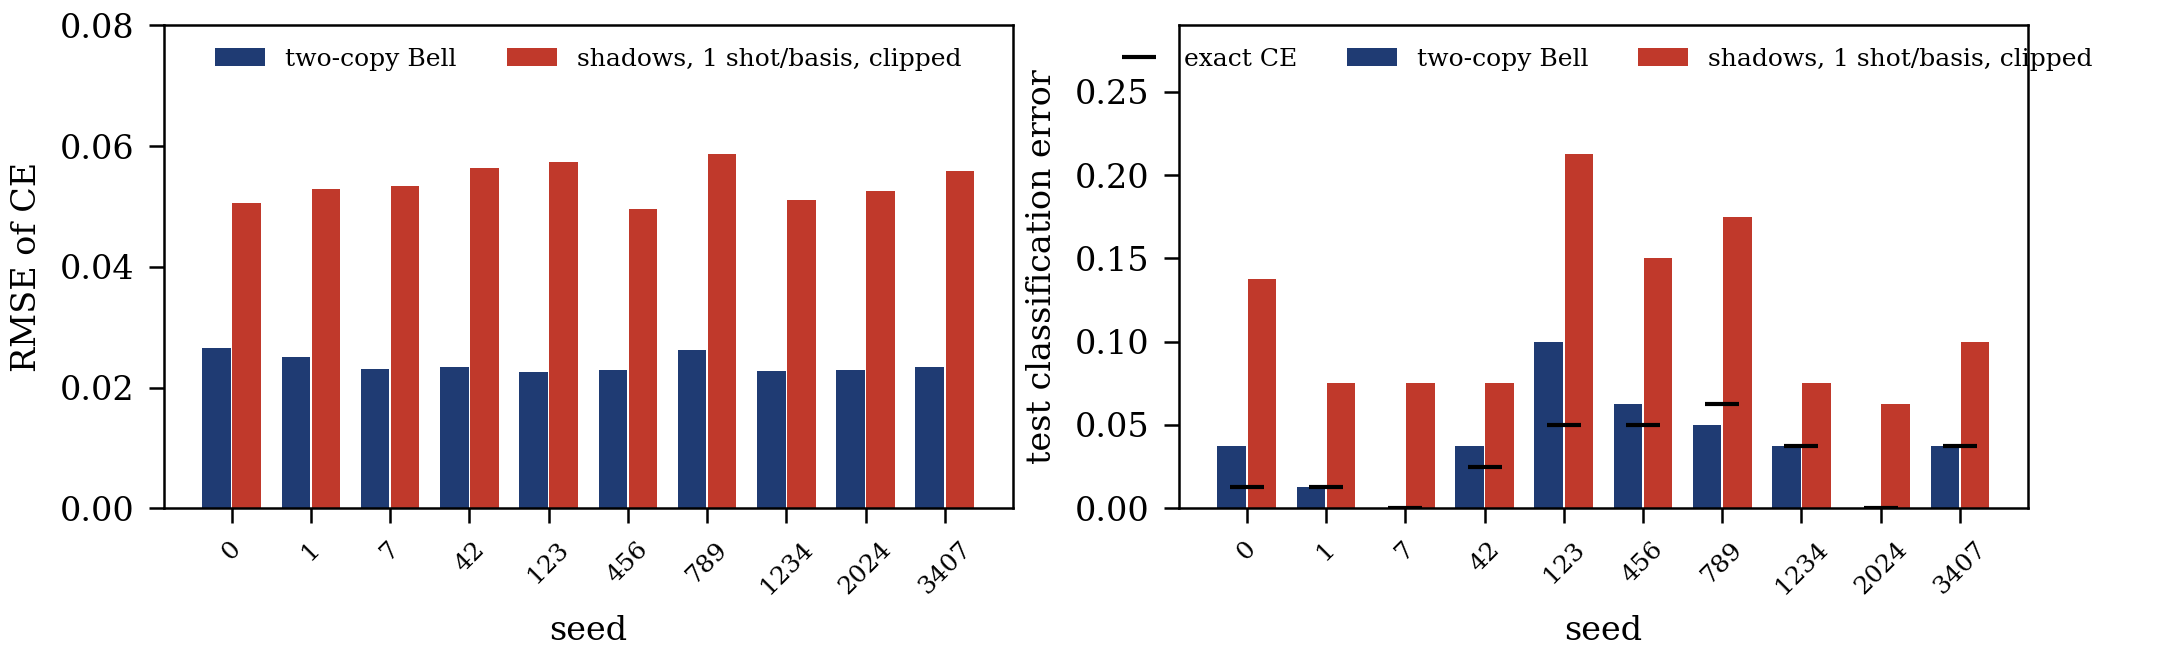
\includegraphics[width=\textwidth]{fig3_ntangled.png}
\caption{NTangled, four qubits, classes with target CE $0.05$ and $0.25$, $C=400$ copies, per
seed. Left: RMSE of the concentratable entanglement. Right: test error of a threshold classifier
on the estimate; black ticks mark the exact CE.}
\label{fig:ntangled}
\end{figure}

\subsection{Noise and an emulated device}

We apply per-qubit depolarising noise $p$ to every qubit of every copy and readout error
$\varepsilon$ to every measured bit, simulated exactly on the raw outcomes (Methods;
Fig.~\ref{fig:noise}, Supplementary Table~\ref{tab:noise}). Depolarising noise biases both readers
by the same amount ($-0.248$ and $-0.244$ at $p=0.10$), as expected from unbiased estimators of the
purity of the noisy state, so noise erodes the coherent reader's relative lead without singling it
out. Uncorrected, it stays ahead in all ten seeds up to $p=0.20$ and $\varepsilon=0.20$, and in
three of ten at $p=0.30$. What separates the readers is calibration: for pure input states the
purity of the whole register is one, so the coherent reader reads its contraction off the same
samples at no cost and inverts it (Methods), whereas the single-copy reader would need the purity
of all $2|A|$ qubits. Self-calibrated, the coherent reader stays ahead in all ten seeds over the
whole grid, by $3.1\times$ at $p=0.10$ and $3.3\times$ at $\varepsilon=0.10$. Memory dephasing has no
effect: purity is invariant under local unitaries and local Paulis map Bell states to Bell states.

\begin{figure}[H]
\centering
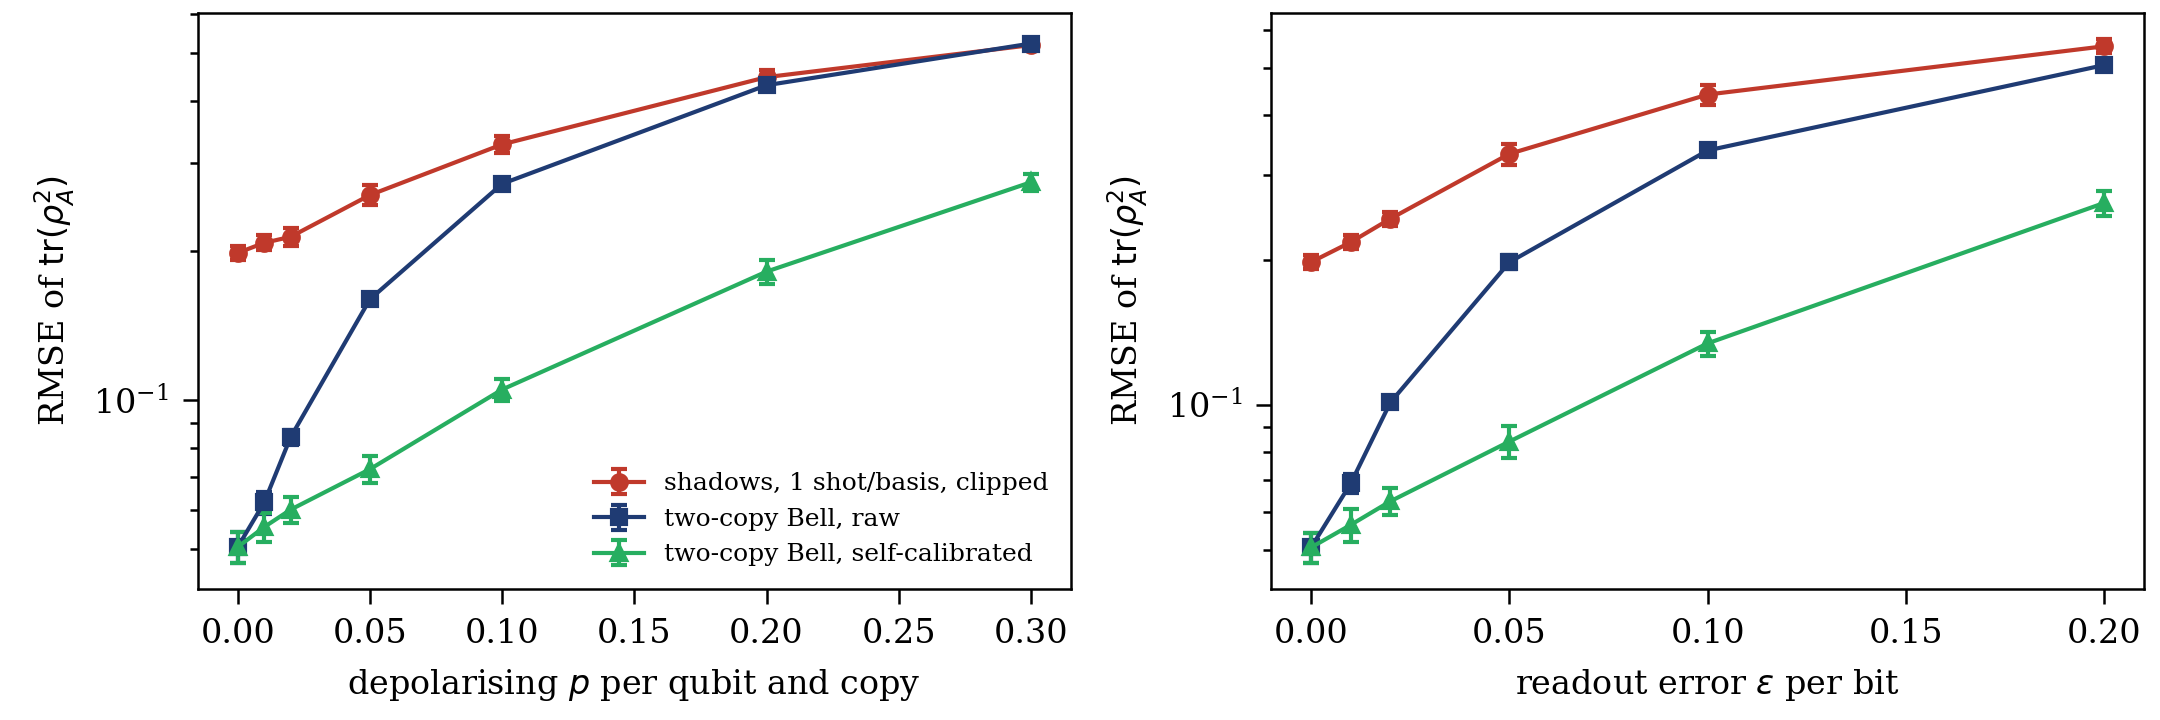
\includegraphics[width=\textwidth]{fig2_noise.png}
\caption{Exact noise at $|A|=4$, $C=400$; mean and s.d.\ over ten seeds. Left: per-qubit
depolarising error on both copies. Right: readout error per measured bit. Noise is simulated on
the raw outcomes and validated against density-matrix calculations (Methods).}
\label{fig:noise}
\end{figure}

To include compilation and a realistic error budget, we transpiled both protocols to the heavy-hex
\texttt{FakeFez} model (156-qubit IBM Heron r2) at optimisation level 3 and simulated them with its
calibrated noise model: gate and readout errors and relaxation and dephasing times, plus the
routing overhead of the connectivity (Methods). The two-copy reader runs on $2n$ physical qubits
with $C/2$ shots; the local single-copy reader runs one random Pauli basis per shot.

\EmulatedBlock

The configuration at $|A|=2$ is the $2\times4$-qubit proof of concept we propose for hardware.
With $100$ states it needs $100$ Bell circuits of $200$ shots and $900$ single-copy circuits sharing
$40{,}000$ shots: $6\times10^{4}$ shots and $10^{3}$ circuits in total, a single short job on current
IBM devices.

% ---------------------------------------------------------------
\section{Discussion}

Coherent two-copy readout is worth a measurable, predictable number of preparations for labels
built from subsystem purities. Against local randomized measurements the number is about three at
$|A|=2$ and about two hundred at $|A|=8$ for our budget; against global random measurements it is
two and about twenty. The comparison is fair in the sense that matters: the budget is in copies,
the single-copy readers are the most copy-efficient configurations we found, local and global, the
learner on top is the same, and the noise is simulated exactly.

The exchange rate is a property of the state ensemble and the budget, not a constant. It follows
from the U-statistic variance decomposition \citep{elben2020mixed} once the two terms are evaluated
for the states at hand rather than bounded, and the bound overstates it four- to fivefold at
our budget and by more than an order of magnitude asymptotically. A practitioner can thus compute the
rate for a target ensemble before deciding to spend qubits on a second copy. Against global
single-copy readers the rate is smaller but still exceeds one at every size, before counting the
entangling circuits across $A$ that those readers need.

The gap is statistical rather than representational. A classical model on all $3^4$ full-support
Pauli expectations represents the purity exactly and still fails at this budget (Supplementary
Table~\ref{tab:rivals}), and the learned tasks show that the gap is not an artefact of thresholding
a single estimate. What our results do not establish is an advantage for labels outside the span
of low-order purities, such as full spectra, where a trainable multi-copy circuit would be the
object of study, nor for labels linear in the state, where single-copy readers are already optimal.
Adaptive single-copy protocols can reach the optimal $\sqrt d$ scaling \citep{liu2026moments}; our
global reader is non-adaptive, so the exchange rate against the best adaptive single-copy protocol
may be lower than the global rates we report.

Three limitations bound the claims. The self-calibration relies on pure input states; for
mixed-state data the anchor disappears. No physical device was used: the noise thresholds and the
emulation are design targets, and the emulated model omits crosstalk, leakage and drift. And the
analyses beyond the confirmatory campaign (Fig.~\ref{fig:scale}, Tables~\ref{tab:learn} and
\ref{tab:emu}) were added after it; they use the official seeds, are labelled exploratory and all
favour the coherent reader in every seed, but they are not covered by the pre-registered test.

Our process should also be stated. The confirmatory endpoint moved from classification error to
estimator RMSE after the single-seed gate and before any confirmatory seed, because development
seeds showed that an $80$-state test split could not resolve the pre-registered margin. An internal
audit after the campaign found that the pre-registered single-copy reader was not the strongest
available and that an earlier noise model, acting on swap signs instead of measured bits, was not
exact and was biased against the coherent reader. Both are corrected here; the campaign is
re-scored against the stronger reader, which only makes the test harder. The first $200$ of the
$400$ states of seed $42$ coincide with the gate's states.

% ---------------------------------------------------------------
\section{Methods}

\subsection{States, seeds and statistics}
Brickwork circuits of depth $d\in\{1,2,3,4\}$, drawn uniformly, with Haar-random two-qubit gates on
a chain of $n=2|A|$ qubits; $A$ is the left half. All results use the ten seeds
0, 1, 7, 42, 123, 456, 789, 1234, 2024 and 3407, fixed before any confirmatory run; development used
seeds $\ge9001$ (Supplementary Table~\ref{tab:rivals}). Per-seed paired differences (coherent minus
strongest single-copy), exact one-sided Wilcoxon signed-rank test, paired $t$ test for
sensitivity, Holm correction over the pre-registered two-idea family, $\alpha=0.05$; ten seeds make
$9.8\times10^{-4}$ the smallest attainable $p$.

\subsection{Two-copy reader}
Each shot measures qubit $q$ of both copies in the Bell basis (CNOT from copy 1 to copy 2, Hadamard
on copy 1, readout of bits $a_q,b_q$). The sign $s_q=(-1)^{a_qb_q}$ is the eigenvalue of the swap
on pair $q$ and $\mathrm{tr}(\rho_W^2)=\mathbb{E}[\prod_{q\in W}s_q]$ for every subset $W$. For
noise-free sweeps we use the exact equivalent that the product over $A$ is a $\pm1$ variable with
mean $p$, i.e.\ $2\,\mathrm{Bin}(C/2,(1+p)/2)/(C/2)-1$; the campaign, noise, learning, NTangled and
emulation experiments sample the full $2n$-qubit Bell distribution.

\subsection{Single-copy readers}
\emph{Local.} $C$ snapshots in $C/S$ random local Pauli bases with $S$ shots each; unbiased
U-statistic over pairs from different bases (same-basis pairs are correlated and excluded). For
noise-free sweeps snapshots restricted to $A$ are drawn from $\rho_A$ directly, which is exact for
local measurements, using the exact outcome table of all $3^{|A|}$ bases computed by contracting
$\rho_A$ qubit by qubit; an oracle checks the table against explicit unitaries and the fast
estimator against the reference implementation (to $10^{-9}$) before every run. \emph{Global.}
One Haar-random unitary on $A$ per shot, snapshot $(d+1)U^\dagger|b\rangle\langle b|U-I$, so
$\mathrm{tr}(\hat\rho_i\hat\rho_j)=(d+1)^2|\langle v_i|v_j\rangle|^2-(d+2)$ with
$v=U^\dagger|b\rangle$ and the U-statistic follows from $\|\sum_iv_iv_i^\dagger\|_F^2$. The observed
$v$ has density $d\langle v|\rho_A|v\rangle$ on the sphere, a mixture over eigenvectors $e_j$ with
weights $\lambda_j$ of densities $d|\langle v|e_j\rangle|^2$, under which
$|\langle v|e_j\rangle|^2\sim\mathrm{Beta}(2,d-1)$; we sample it exactly in $O(d)$ per shot and check
it against explicit Haar unitaries and a rejection sampler. All estimates are clipped to
$[2^{-|A|},1]$.

\subsection{Exchange rates}
Copies to match the coherent reader at $C=400$ are measured on a grid of budgets ($C$ doubling from
$100$) and interpolated in log--log, never extrapolated. For the exact prediction, the snapshot
distribution $P(x)$ over $x=(b_q,o_q)_{q\in A}$ ($6^{|A|}$ symbols) is computed by contracting
$\rho_A$ with the basis rotations. With the single-qubit kernel $T$ ($5$ for equal basis and
outcome, $-4$ for equal basis and different outcome, $1/2$ otherwise), $g=T^{\otimes|A|}P$,
$p=P^\top g$, $\zeta_1=P^\top g^2-p^2$ and $\zeta_2=P^\top(T^{\circ2})^{\otimes|A|}P-p^2$. The
formula Eq.~\eqref{eq:var} is checked against $4000$ Monte Carlo repetitions before every run
(within $8\%$). The bound-implied rate replaces $4\zeta_1/M+2\zeta_2/M^2$ by
$4\cdot2^{|A|}p/M+4\cdot8^{|A|}/M^2$ (Eq.~D16 of Ref.~\citenum{elben2020mixed}).

\subsection{Noise and self-calibration}
Depolarising error $p$ on a qubit is a uniformly random Pauli, each with probability $p/4$; through
the Bell circuit $X$ on either copy flips $b_q$, $Z$ flips $a_q$, $Y$ flips both. Readout flips each
bit with probability $\varepsilon$. For the local reader a depolarised qubit gives a uniform outcome
and readout flips the bit. Both models act on raw outcomes of clean samples, which is exact for
these channels, and agree with density-matrix calculations on $n=2$ to within $7\times10^{-4}$. We
model the contraction as $\mathbb{E}[\hat p_W]\approx\lambda^{|W|}p_W+(1-\lambda^{|W|})2^{-|W|}$,
estimate one global $\lambda$ from the full-register Bell purity,
$\lambda=\big((\overline{\hat p}_{\mathrm{full}}-2^{-n})/(1-2^{-n})\big)^{1/n}$, and invert for $A$.
A per-state $\lambda$ amplifies calibration noise and is not used; without noise the correction is
the identity.

\subsection{Learned labels}
Pre-registered in \texttt{exp\_bell\_learn.py} before any run; development seed $9501$ only checked
that the pipeline executes. $n=8$, $400$ states per seed, $240/160$ split, $C=400$ copies per state
for every reader. Features: the $26$ contiguous window purities of width $1$ to $4$, clipped, and
their logarithms; the local-Pauli baseline uses all weight-$\le2$ expectations from the same
snapshots. L1: multinomial logistic regression ($C=1$); L2: ridge regression ($\alpha=1$);
standardised features, no hyperparameter search.

\subsection{NTangled}
Weights from \texttt{LSchatzki/NTangled\_Datasets}, hardware-efficient ansatz, four qubits, depth
three: per layer $U3$ on every qubit, CZ on $(2i,2i+1)$, $U3$ again with the same angles, CZ on
$(2i+1,2i+2)$, with $U3(\theta,\phi,\lambda)=R_z(\phi)R_x(-\pi/2)R_z(\theta)R_x(\pi/2)R_z(\lambda)$.
Inputs are product states with real amplitudes, which reproduce the target CE of each class (exact
means $0.049$ and $0.252$ for the classes labelled $0.05$ and $0.25$). One hundred states per class,
$60/40$ split, logistic regression on the scalar CE estimate.

\subsection{Device emulation}
\texttt{FakeFez} from \texttt{qiskit-ibm-runtime} and \texttt{NoiseModel.from\_backend} in Aer;
transpilation at level $3$ with the seed as transpiler seed. One shot per random basis is
implemented exactly by drawing the $C$ basis labels first and running each distinct basis with its
multinomial count. Bell and single-copy circuits are simulated in separate batches with an explicit
method: a single batch mixing them returned near-constant outcomes for the single-copy circuits,
while each circuit alone was correct. A noiseless run of the same pipeline reproduces the ideal
results (Table~\ref{tab:emu}).

% ---------------------------------------------------------------
\section*{Data availability}
NTangled generator weights are public (\url{https://github.com/LSchatzki/NTangled_Datasets}). All
other data are generated from the listed seeds; per-seed results are in \texttt{results/bell\_qnn/}.

\section*{Code availability}
\begin{sloppypar}
Repository \texttt{qdata-gates}: \texttt{exp\_bell\_qnn.py} (gate and campaign),
\texttt{exp\_bell\_paper.py} (scaling, copies, noise, NTangled), \texttt{exp\_bell\_global.py}
(global reader and bound), \texttt{theory\_bell.py} (exact variances), \texttt{exp\_bell\_learn.py}
(learned labels), \texttt{exp\_bell\_emulated.py} (device emulation), \texttt{qdlib.py}
(estimators), \texttt{audit\_*.py}, \texttt{fig\_paper.py} and \texttt{fill\_macros.py}, which
writes every swept number in this manuscript from the result files.
\end{sloppypar}

\section*{Author contributions}
% TODO(authors)
To be completed.

\section*{Competing interests}
The authors declare no competing interests.

\bibliographystyle{unsrtnat}
\bibliography{references}

% ---------------------------------------------------------------
\clearpage
\section*{Supplementary information}
\renewcommand{\thetable}{S\arabic{table}}
\setcounter{table}{0}

\begin{table}[H]
\centering
\small
\caption{Development comparison of single-copy readers: classification error at $C=400$ copies,
mean over ten development seeds, $80$ test states each, local readers with $S=10$. The coherent
reader is a logistic regression on all Bell window purities. A classical model on all $3^4$
full-support Pauli expectations represents the purity exactly,
$\mathrm{tr}(\rho_A^2)=2^{-|A|}\sum_P\langle P\rangle^2$, and still fails at this budget. Grouping
also costs accuracy: the purity RMSE at $|A|=4$ was $0.332$ ($S=10$), $0.274$ ($S=5$), $0.245$
($S=2$) and $0.234$ ($S=1$), and clipping lowered the last to $0.202$.}
\label{tab:rivals}
\begin{tabular}{lr}
\toprule
Reader & Test error \\
\midrule
Two-copy Bell, window purities & \textbf{0.086} \\
Shadows, window purities (U-statistics) & 0.135 \\
Shadows, local Pauli $k\le2$, logistic & 0.494 \\
Shadows, full support on $A$ ($3^4$ chains), logistic & 0.519 \\
Shadows, full support on $A$, SVM-RBF & 0.403 \\
Inverted shadow density matrix, $\mathrm{tr}(\hat\rho_A^2)$ & 0.256 \\
Hybrid: U-statistic purity + full-support chains & 0.404 \\
\bottomrule
\end{tabular}
\end{table}

\begin{table}[H]
\centering
\small
\caption{Noise study, $|A|=4$, $C=400$, mean over ten seeds. ``Wins'' counts seeds in which the
coherent reader (raw / self-calibrated) has lower RMSE than the strongest local single-copy reader.}
\label{tab:noise}
\setlength{\tabcolsep}{4pt}
\begin{tabular}{llrrrrrr}
\toprule
Channel & Level & Bell & Bell cal. & Single & Bias Bell & Bias single & Wins \\
\midrule
none & 0 & 0.051 & 0.051 & 0.198 & $+0.001$ & $-0.038$ & 10 / 10 \\
depolarising & 0.02 & 0.084 & 0.060 & 0.213 & $-0.059$ & $-0.084$ & 10 / 10 \\
depolarising & 0.05 & 0.160 & 0.073 & 0.259 & $-0.139$ & $-0.149$ & 10 / 10 \\
depolarising & 0.10 & 0.273 & 0.105 & 0.328 & $-0.248$ & $-0.244$ & 10 / 10 \\
depolarising & 0.20 & 0.431 & 0.182 & 0.448 & $-0.398$ & $-0.381$ & 10 / 10 \\
depolarising & 0.30 & 0.523 & 0.275 & 0.519 & $-0.485$ & $-0.456$ & 3 / 10 \\
readout & 0.02 & 0.101 & 0.063 & 0.244 & $-0.078$ & $-0.128$ & 10 / 10 \\
readout & 0.05 & 0.198 & 0.084 & 0.332 & $-0.175$ & $-0.249$ & 10 / 10 \\
readout & 0.10 & 0.338 & 0.134 & 0.441 & $-0.309$ & $-0.376$ & 10 / 10 \\
readout & 0.20 & 0.508 & 0.263 & 0.556 & $-0.470$ & $-0.497$ & 10 / 10 \\
\bottomrule
\end{tabular}
\end{table}

\end{document}
